\chapter{Änderungen durch neue Antriebe, Annahmen und Methodik}
\label{ch:Änderungen durch neue Antriebe, Annahmen und Methodik}

Konzepte mit neuen Antrieben befinden sich im Entwicklungsprozess und bis jetzt es ist ratsam, wie zukünftige Flughäfen aussehen werden
und welche Ausstattung für die Flugzeug-Abfertigung ausgesucht wird. Wasserstoff-Flugzeuge werden erst ab dem Jahr 2035 in 
auf den Markt eintreten, wobei die BA-Flugzeuge schon in den nächsten Jahren erwartet werden.
Der Wechsel zu nachhaltigen Antrieben kann es zu deutlichen Änderungen in der Infrastruktur und Abläufen am Vorfeld führen, die
in diesem Kapitel beschrieben werden.
Außerdem auf der Grundlage der unterschiedlichen Quellen und vernünftigen Behauptungen wird eine Reihe der Annahmen für diese Arbeit getroffen.
%Dieser Teil der Arbeit beschäftigt sich mit der vorhandenen Infrastruktur-Optionen. %und im Fall des Wasserstoffs Lieferketten.
%
%Wenn die Infrastruktur auf den Regionalflughäfen gemacht wird, 
%macht es nicht so ein Ausmaß wie auf größeren Flughäfen, wo viele Abfertigungsplätze umgerüstet werden müssen.

\section{Änderungen an der Abfertigung und dazugehörige Kosten von alternativen Antrieben}
\label{s:Änderungen an der Abfertigung und dazugehörige Kosten von alternativen Antrieben}

Infrastrukturkosten sind von der Größe des Flughafens abhängig. Größere Flughäfen können mehr Flugzeuge als Regionalflughäfen 
abfertigen, was dazu führt, dass mehr Abfertigungsplätze umgerüstet und versorgt werden müssen und mehr Arbeitskräfte geschult werden müssen. 
In diesem Teil wird näher auf die Änderungen in der Infrastruktur durch die Einführung von neuen Antrieben eingegangen und 
die Forschungsrichtung ausgesucht.

\subsection{SAF}
SAF ist zwar nicht die beste langfristige Lösung wegen vorhandenen Emissionen, aber wegen benötigter Entwicklung der anderen nachhaltigen
Antrieben stellt eine gute Option dar. In der nahen Zukunft werden vor allem die großen Flugzeuge mit BA-Antrieb nicht entwickelt, 
deswegen können SAF für die Langstreckenflüge benutzt werden \cite{dalmia2022powering}.
Diese Arbeit wird sich auf das reine SAF ohne Beimischung beschränken, da nur so das gesetzte Ziel bis zum Jahr 2050 erreicht werden kann.

SAF benötigt keine Infrastrukturänderung und darf in bestehenden Systemen und Flugzeugen benutzt werden \cite{dalmia2022powering}.
Dadurch, dass SAF zu herkömmlichen Treibstoffen beigemischt wird, ist zurzeit einen zusätzlichen Treibstofftank 
für das gemischten Kraftstoff gebraucht. Bis jetzt Transport von SAF mit einer Pipeline nicht zugelassen (Quelle?).
Bei der intensiven Recherche wurde jedoch keine Information gefunden, die besagt, dass es verboten wird reine SAF nicht als
Drop-In zu benutzen. Aus diesem Grund gilt für die Arbeit, dass die Lieferung von SAF mit bestehenden Pipelines 
zertifiziert und genauso wie bei Betankung mit herkömmlichen Treibstoffen zugelassen wird.

\subsection{Batterie-Antrieb}
Batteriegetriebene Flugzeuge brauchen größere Veränderung am Flughafen als bei der Nutzung von SAF.
Bis zum Jahr 2050 sind die BAs auf die kleineren Flugzeuge und damit auf Kurz- und Regionalverkehr beschränkt. 

In der Literatur werden zwei Batterien-Lademöglichkeiten diskutiert, die Batterien zu wechseln (Swap-Methode), 
wo die Batterie aus dem Flugzeug herausgenommen werden und 
an einer Ladestation geladen, oder Ladekabel in das Flugzeug einzustecken (Plug-In), wie bei etablierten E-Autos.
%
Bei diesem Antrieb muss beachtet werden, welche Lebensdauer eine Batterie hat und wie die Batterien geladen werden. 
Je länger die Ladung dauert, desto mehr Kosten auf dem Boden verursacht werden. Nichtsdestotrotz kann schnelle Ladung 
zur Stagnation von Lebensdauer einer Batterie bringen (Quelle).

Ladeleistung ist für die Dauer der Ladung verantwortlich. Durch schnellere Ladungen wird Lebensdauer der Batterien reduziert. 
Was mit sich bringt, dass die Batterien schneller ausgetauscht werden müssen
und mehr Kosten dadurch entsteht. (Quelle) Wobei die langsamen Laden ist für die Fluggesellschaften nicht rentabel sein kann, 
da wenn Flugzeug auf dem Boden steht verdienen Fluggesellschaften kein Geld.


\textit{Plug-In} Methode benötigt ein schnelles Laden, damit Flugzeuge weniger Zeit auf Boden verbringen müssen.
Jedoch ist ein Anstieg in Turnaround-Zeiten aufgrund nicht zurzeit möglichen Schnellladung möglich \cite{avogadro2024demystifying}.

Bei \textit{Swap-Methode} kann Aus- und Einbau der Batterie aus dem/in das Flugzeug lange dauern \cite{dalmia2022powering}. 
Guo et al. \cite{guo2020aviation} ist zum Schluss gekommen, dass Batteriewechsel effizienter und ökonomischer ist, 
wenn die batteriebetriebenen Flugzeuge nur ein kleiner Teil (unter 10 \%) der Flotte ist, in anderem Fall lohnt sich eine Plug-In-Ladung. 
Für die Batteriewechsel müssen auch Transport und Hebegeräte gestellt werden, um die Batterien bewegen zu können \cite{reimers2018introduction}.
Jedoch mit Batteriewechsel können die Abfertigungszeiten reduziert werden (Quelle), was an einem großen Flughafen von der Bedeutung ist. 

Batteriewechsel bietet gleichmäßigere Deckung der Nachfrage \cite{guo2020aviation} und kompatibler mit der Flugplanung \cite{salucci2020optimal}, 
da der Austausch einer Batterie viel schneller ist, als Dauer einer Plug-In Ladung. 
Jedoch werden mehrere Batterien benötigt, die zudem ordnungsgemäß und sicher gelagert werden müssen \cite{salucci2020optimal}.
Außerdem ermöglicht der Swap-Methode langsameres Laden und macht das Laden mit geringer Leistung möglich \cite{avogadro2024demystifying}.
Aus diesen Gründen werden in nächsten Teilen die Kosten für diese Option ausgewertet. 

Würde der Austausch der Batterien parallel zu anderen Prozessen, wie Deboarding kann die kürzere Turnaround-Zeit im 
Vergleich zu konventionellen Flugzeugen erreicht werden \cite{schmidt2016challenges}.

\textit{Annahmen für die BA-Analyse}\\

Für weitere Betrachtung wurde es die Swap-Methode entschieden. Zudem wird es angenommen, 
dass die Batterien für Flugzeuge zur Flughafen-Infrastruktur gehören.
Das bedeutet, dass diese Anschaffungskosten für Flughafen anfallen und danach werden sie in Form von Leasing 
von für Fluggesellschaften ausgeliehen.

Für die Ladevorgänge wird Strom benötigt. 
Die Strompreise und die vorhandene Leistung sind normalerweise von Tag und Nacht abhängig \cite{salucci2020optimal}, 
aus praktischen Gründen wird die konstante Spitzenleistung von Batteriewechselsystem von 250 kW wird angenommen. 
Bei einer Batteriekapazität von 900 kWh, würde die Ladung bei so einer Leistung ohne Beachtung der Verluste 3,6 Stunden dauern.

%
Für die Nachhaltigkeit des Batterieantriebes sind die Energiequellen von der Bedeutung. 
Der Strom aus dem Stromnetz kann sein Ursprung aus den Kraftwerken und Verteilerzentren haben \cite{dalmia2022powering}. 
Was dazu führt, dass die fossilen Brennstoffe für die Verbrennung benutzt werden und dadurch zu Emissionen beitragen. 
Als Alternative wäre Nutzung der erneuerbaren Energiequellen, wie Windenergie oder Solarenergie. Diese Energie ist normalerweise teurer
und die Produktionsmenge ist bis jetzt nicht ausreichend, um die Luftverkehr-Nachfrage zu decken (Quelle).
Anstieg in Turnaround-Zeiten aufgrund nicht zurzeit möglichen Schnellladen möglich \cite{avogadro2024demystifying}.
%Für die Ladung den batteriegetriebene-Flugzeugen Infrastruktur:
%Infrastrukturmodell nach Guo et al. "Die EA-Aufladung wird teilweise von einer flughafenbasierten Solar-PV-Anlage geliefert.
%Jährliche Betriebskosten (OPEX)= Strombezugskosten aus dem Netz in der Sommer und Wintersaison (typische Tage) basierend auf der Nachfrage. \cite{guo2020aviation}
Zudem ist ein modulares System möglich, wo beide Ansätze benutzt werden \cite{salucci2020optimal}.

\subsection{Wasserstoff}
Logistik ist ein wichtiger Teil der Produktionskette. 
Die Nutzung des Wasserstoffs am Flughafen erfordert Austausch der Betankungsanlagen und Anschaffung neuen Lieferketten, 
um Wasserstoff als Treibstoff benutzen zu können. Diese Investitionskosten werden die Flughafenbetreiber beeinträchtigen. 
\textit{Transport}\\
Die Lieferketten und die Produktion des Wasserstoffs haben ein großes Gewicht in der vorhandenen Literatur.
Der Transport ist durch Pipelines im gasförmigen Zustand, LKW und Zügen sowohl im gasförmigen, als auch im flüssigen Zustand möglich. 
Kapitel \ref{ss:Wasserstoff-Antrieb} stellte die möglichen physischen Formen von Wasserstoff dar und am Ende darlegte,
dass flüssiger Wasserstoff für den Transport als im Gasform vorteilhafter ist. 
Außerdem kann es auch in einer chemischen Verbindung, wie Ammoniak und Methanol, gebunden und somit transportiert werden.
%
%
%Wasserstoff kann hochentzündlich sein \cite{dalmia2022powering}. %(prüfen ob entzündlicher als Kerosin)
%
% 
Die Effizienz der Produktion- und Lieferkosten ist geografisch determiniert. 
Die Lieferoptionen sind nach Flughafenposition zu wählen. Für die Flughäfen, die nahe einer Wasserstoff-Pipeline liegen ist sinnvoller
damit der Wasserstoff zu besorgen, als mit einem LKW transportieren zu lassen.
%
Für europäische Distanzen sind die Wasserstoff-Pipelines günstiger als Transport mit chemischen Verbindungen, 
welcher bei längeren Distanzen in Betracht kommt \cite{undertaking2022strategic}. 
Bei Änderung von Erdgasleitung für Wasserstoff können Kosten gespart
werden und muss keine neue Infrastruktur gebaut werden, sondern die Leitungen für Wasserstoff umgerüstet werden können \cite{undertaking2022strategic}.

Der Transfer von \ce{LH2} mit vakuumisolierte Pipeline beschränkt sich auf die kurzen Distanzen
wegen proportionalen Skalierung der Verluste zu Leitungslänge \cite{colpan2022fuel}.

Colpan et al.\cite{colpan2022fuel} ist der Meinung im Fall, wenn große Menge an Wasserstoff benötigt wird, 
ist der Lieferung weder LKW noch Pipeline sinnvoll. 

Dennoch nach Schenke et al. \cite{schenke2024lh2} kann Lieferung den flüssigen Wasserstoff mit einem LKW bei einer hohen Anzahl an Flügen 
kostengünstiger als andere Lieferalternativen sein. Allerdings Transport von \ce{LH2} erfordert speziell konstruierte Tanks \cite{mulder2019outlook}.

Lieferung von gasförmigem Wasserstoff mit niedrigem Druck mit dem Straßenverkehr bis jetzt nur für ungenügende Menge möglich \cite{undertaking2022strategic}

Obwohl die hohen Kapitalkosten von Pipeline-Anlage zu erwarten, die Betriebskosten niedriger sein werden \cite{mulder2019outlook}. Also bei größerem Umfang lohnt es Pipelines, sonst Lkw \cite{mulder2019outlook}.

\textit{Speicherung}\\
Gasförmiger Wasserstoff kann unterirdisch in Salzkavernen und in erschöpften Gasfelder gespeichert werden \cite{undertaking2022strategic}, 
Sie müssen sich in der unmittelbaren Nähe zum Flughafen befinden. Da es sich je nach Flughafenstandort variiert, wird dieser Speicheroption nicht weiter behandelt.
Außerdem kann es für die Lagerung ein oberirdischer Druckzylinder, wo flüssiger Wasserstoff oder als festen Materialien (wie Metallhybriden) gespeichert wird.
Aufgrund tiefen Temperaturen müssen diese Zylinder oder Tankern müssen gut isoliert und kryogen sein \cite{undertaking2022strategic}.
Andernfalls wird flüssiger Wasserstoff bei der Lagerung verdampft, was zum Verlust der Menge kommt \cite{undertaking2022strategic}. 
Die Verdampfung wird mit größeren Lager kleiner \cite{colpan2022fuel}.

Dennoch der größte Teil der Verdampfung findet durch Transferphase statt \cite{undertaking2022strategic}.
%Wasserstoff kann in Hochdrucktanks und Salzkavernen gelagert werden \cite{mulder2019outlook}
Somit muss der Weg zwischen Betankung und dem Speicher kurz sein, damit Verdampfungsverluste minimiert werden können \cite{colpan2022fuel}


Eine weitere mögliche Betankungsoption ist der Austausch des Flugzeugtanks als Kapseln. Dabei werden die leeren Kapseln an die 
Wasserstoffproduktionsstelle zurückgegeben, wo die wieder nachgefüllt werden können \cite{colpan2022fuel}. 
Diese Möglichkeit kann vor allem für die kleineren Flughäfen als Alternative sein, da kein Wasserstoffspeicher und 
sonstige Anlagen bereitgestellt werden müssen.
Für längeres Parken am Flughafen werden kalte Tanks eine sichere Verbindung mit der Wasserstoffinfrastruktur benötigen \cite{colpan2022fuel} %weiß nicht
Grund?
%"current FCEV system costs higher than 200 €/kW for passenger cars but need 
%to fall below 50 €/kW for mass market. " \cite{undertaking2022strategic}


%neue terminals: In dem Fall, falls die Flugzeuge länger als übliche Modelle werden, die Sicherheitssperzone für die Betankung 20 Meter betragen kann \cite{gu2023hydrogen}
%
%
%"Flüssiger Wasserstoff muss jedoch bei Minusgraden gelagert werden, was eine Verbesserung der Speichertechnologien sowohl im Flugzeug selbst als auch auf Flughäfen erfordert."
%Wasserstoff kann entweder als Brennstoff für Verbrennung genutzt werden oder als Wasserbrennstoffzelle für die elektrischen Flugzeuge. \cite{dalmia2022powering}

In dem Unterkapitel \ref{Wasserstoff-Antrieb} wurde angeführt, dass die Produktion des Wasserstoffs, 
viel Platz Energie und hohe Kosten benötigt. Produktion und Verflüssigung des Wasserstoffs am Flughafen würde viel zusätzliche Infrastrukturkosten \cite{dalmia2022powering}.
Deswegen für die Flughäfen wäre es die Alternative besser, das Wasserstoff, woanders einzukaufen und zum Flughafen 
mit LKW oder Pipelines liefern zu lassen \cite{gu2023hydrogen}.
Aufgrund aufwendigeren und kostenintensiven Infrastrukturprozessen für die Produktion und Verflüssigung von 
Wasserstoff werden wahrscheinlich Flughäfen, 
besonders kleineren, anfangs auf die "On-Site" Produktion verzichten.

Aufgrund hohen Unterschiedes zu herkömmlichen Treibstoffen und neuen Ausrüstungen müssen die Mitarbeiter neu geschult werden, 
um mögliche Gefahren zu erkennen und zu vermeiden \cite{gu2023hydrogen}.

%In der Arbeit Dalmia et al. \cite{dalmia2022powering} wird die Produktion am Flughafen diskutiert. 
%Dazu wird einen Elektrolyseur für Erzeugung des gasförmigen Wasserstoffs, einen Kompressor und einen Tankwagen oder
%eine Pipeline mit modularem Tanksystem für Betankung der Flugzeuge benötigt. 
%Modulares Tanksystem kann in bestehenden Flugzeugen eingesetzt werden
%und wird als wie Fracht in das Flugzeug geladen. %(nochmal nachlesen)
%
%Für die Wasserstofferzeugung wäre die ideale Methode der Elektrolyse, die mit Strom betrieben würde, der vor Ort aus 
%erneuerbaren Ressourcen erzeugt würde, wie z. B. Solarenergie aus nicht reflektierenden Paneelen (um eine Blendung der 
%Solarmodule für Piloten zu vermeiden). Das Wasser, das für den Prozess verwendet wird, wird aus nahe gelegenen 
%Wasserquellen stammen, einschließlich Süßwasserflüssen und Seen. Diese Wasserstoffproduktion wird vor Ort an Flughäfen 
%stattfinden. Die benötigte Infrastruktur umfasst einen Elektrolyseur, einen Kompressor und einen Tankwagen. 
%Der Elektrolyseur wird gasförmigen Wasserstoff erzeugen. Der Kompressor erhöht dann den Druck des Wasserstoffs, 
%indem er sein Volumen für die Speicherung reduziert, und der Tankwagen transportiert den komprimierten Wasserstoff 
%zum Elektroflugzeug. Eine weitere Option für den Transport wäre die Installation einer landseitigen bis luftseitigen Pipeline,
% die den komprimierten gasförmigen Wasserstoff in einem modularen Tanksystem transportiert. Dieses System ermöglicht 
% die Nachrüstung von bereits im Einsatz befindlichen Flugzeugen. Die Wasserstofftanks würden ähnlich wie Fracht 
% in ein Flugzeug geladen, festgeschnallt und sicher mit dem Flugzeug verbunden. Wenn das Ziel erreicht ist, 
% wird der leere Tank durch einen neuen Tank ersetzt, der dann zurückgeschickt wird, um in der Wasserstoffproduktionsanlage 
% am Flughafen wieder aufgefüllt zu werden. Dieses System ermöglicht den Einsatz von Wasserstoff in allen Bereichen des Fluges,
% wodurch die Effizienz maximiert, das Gesamtgewicht reduziert und die Nutzlast und Reichweite verbessert werden.²³\cite{dalmia2022powering}
%
%Gerade wird Wasserstoff durch die Pipelines transportiert \cite{mulder2019outlook}. ist es so?
%Der Transport ist durch Pipelines im gasförmigen Zustand, LKW und Zügen sowohl im gasförmigen,
% als auch im flüssigen Zustand möglich. 
% Transport von LH2 erfordert speziell konstruierte Tanks \cite{mulder2019outlook}

%"Eine Kryopumpe 
%bringt den Wasserstoff auf den benötigten Druck von 1000 bar. " ?file:///C:/Users/henri/Downloads/765438.pdf

\textit{Annahmen für die Analyse}
Die Gesamtinvestitionen sind von der Wahl der Produktion, Speicherung, Lieferketten als auch Betankungsentscheidung abhängig.
Da derzeit nicht einsehbar ist, welcher Technologie umgesetzt wird, fokussiert sich die Arbeit auf einen bestimmten Versorgungsweg.

Die externe Produktion ist am Anfang sinnvoll \cite{colpan2022fuel}, aus diesem Grund wurde angenommen, dass die Produktion 
des Wasserstoffes und Verflüssigung nicht am Flughafen stattfindet, sondern eingekauft und zum Flughafen mit LKW transportiert.
Am Flughafen wird der Wasserstoff in kryogenen Tanks gespeichert und mit Betankungswagen werden die Flugzeuge mit Kraftstoff befüllt.
%
Lieferkosten für flüssigen Wasserstoff \ce{LH2} werden nicht explizit ausgerechnet,
da die schon in Betriebskosten von Wasserstoffbetriebenen Flugzeuge eingeschlossen sind.
%
Die Abbildung \ref{supply_wasserstoff} stellt so eine Variante von Produktion- und Lieferketten für flüssigen Wasserstoff dar.
\begin{figure}[h]
	\centering
	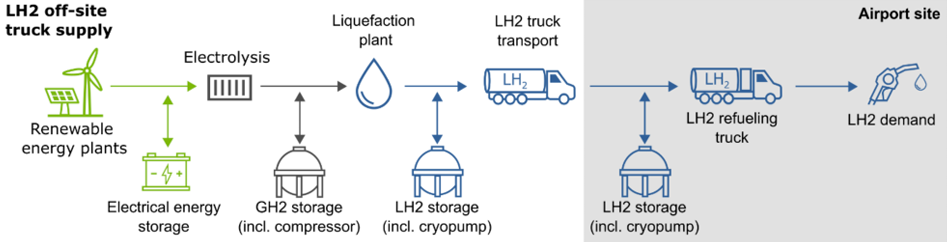
\includegraphics[width=0.9\linewidth]{Bilder/Supply_hydrogen.png}
	\caption[Lieferkette von flüssigem Wasserstoff mit externer Herstellung und interner Lagerung bzw. die Betankung]{Lieferkette von flüssigem Wasserstoff mit externer Herstellung und interne Lagerung bzw. die Betankung \cite{schenke2024lh2}}
	\label{supply_wasserstoff}
\end{figure}

Zusätzlich wird es davon ausgegangen, dass Sicherheitsradius beim Wasserstoffbetankung nicht erweitert wird.
